% !TEX encoding = UTF-8 Unicode
\documentclass[a4paper]{article}

\usepackage{color}
\usepackage{url}
\usepackage[T2A]{fontenc} % enable Cyrillic fonts
\usepackage[utf8]{inputenc} % make weird characters work
\usepackage{graphicx}

\usepackage[font=small,labelfont=bf]{caption}
\usepackage[english,serbian]{babel}
%\usepackage[english,serbianc]{babel} %ukljuciti babel sa ovim opcijama, umesto gornjim, ukoliko se koristi cirilica

\usepackage[unicode]{hyperref}
\hypersetup{colorlinks,citecolor=green,filecolor=green,linkcolor=blue,urlcolor=blue}

\usepackage{listings}

%\newtheorem{primer}{Пример}[section] %ćirilični primer
\newtheorem{primer}{Primer}[section]

\definecolor{mygreen}{rgb}{0,0.6,0}
\definecolor{mygray}{rgb}{0.5,0.5,0.5}
\definecolor{mymauve}{rgb}{0.58,0,0.82}

\lstset{ 
  backgroundcolor=\color{white},   % choose the background color; you must add \usepackage{color} or \usepackage{xcolor}; should come as last argument
  basicstyle=\scriptsize\ttfamily,        % the size of the fonts that are used for the code
  breakatwhitespace=false,         % sets if automatic breaks should only happen at whitespace
  breaklines=true,                 % sets automatic line breaking
  captionpos=b,                    % sets the caption-position to bottom
  commentstyle=\color{mygreen},    % comment style
  deletekeywords={...},            % if you want to delete keywords from the given language
  escapeinside={\%*}{*)},          % if you want to add LaTeX within your code
  extendedchars=true,              % lets you use non-ASCII characters; for 8-bits encodings only, does not work with UTF-8
  firstnumber=1000,                % start line enumeration with line 1000
  frame=single,	                   % adds a frame around the code
  keepspaces=true,                 % keeps spaces in text, useful for keeping indentation of code (possibly needs columns=flexible)
  keywordstyle=\color{blue},       % keyword style
  language=Python,                 % the language of the code
  morekeywords={*,...},            % if you want to add more keywords to the set
  numbers=left,                    % where to put the line-numbers; possible values are (none, left, right)
  numbersep=5pt,                   % how far the line-numbers are from the code
  numberstyle=\tiny\color{mygray}, % the style that is used for the line-numbers
  rulecolor=\color{black},         % if not set, the frame-color may be changed on line-breaks within not-black text (e.g. comments (green here))
  showspaces=false,                % show spaces everywhere adding particular underscores; it overrides 'showstringspaces'
  showstringspaces=false,          % underline spaces within strings only
  showtabs=false,                  % show tabs within strings adding particular underscores
  stepnumber=2,                    % the step between two line-numbers. If it's 1, each line will be numbered
  stringstyle=\color{mymauve},     % string literal style
  tabsize=2,	                   % sets default tabsize to 2 spaces
  title=\lstname                   % show the filename of files included with \lstinputlisting; also try caption instead of title
}

\begin{document}

\title{Optimizacija kolonijom mrava\\ 
\hfill \break
\small{Seminarski rad u okviru kursa\\Naučno izračunavanje\\ Matematički fakultet}}

\author{Vojkan Cvijović, Gorana Vučić\\ vojkan94@ymail.com , goranavucic94@gmail.com}

%\date{9.~april 2015.}

\maketitle

\abstract{


\tableofcontents

\newpage

\section{Uvod}
\label{sec:uvod}

Algoritam optimizacije kolonijom mrava proučava ponašanje mravljih kolonija, u svrhu rešavanja optimizacionih
problema, gde se kao najčešći problem javlja pronalaženje najkraćeg puta u zadatom grafu.

\vspace{3mm}

Pojam ACO (eng.~{\em ant colony optimization}), kao rezultat istraživanja pristupa kombinatornoj optimizaciji, uveo je Marco Dorigo 1992. godine u svom doktoratu. Algoritam se na samom početku primenjivao na problem trgovačkog putnika, a kasnije se sama ideja proširivala i na neke druge probleme.

\vspace{3mm}

Algoritam ACO pripada klasi algoritama inteligencije roja (eng.~{\em Swarm intelligence}). Naime akcije insekata se temelje na interakcijama među pojedincima. Iako te interakcije izgledaju primitivno, globalno gledano često daju dobre rezultate. Takvo kolektivno ponašanje se naziva inteligencija roja. Glavne prednosti jesu fleksibilnost, u smislu brzog prilagođavanja promenljivoj okolini, potom robusnost što predstavlja otpornost na manja odstupanja, kao i sposobnost funkcionisanja bez nadzora. Optimizacija pomoću kolonije mrava je algoritam koji se koristi za nalaženje optimalnih putanja u potpuno povezanom grafu.

\section{Ponašanje mrava}
\label{sec:ponasanjemrava}

Kako je navedeni algoritam nastao po uzoru na ponašanje iz prirode, neophodno je objasniti sam princip rada na stvarnom ponašanju. Ukoliko postavimo mrave u neku nepoznatu okolinu, kako bi pronašli izvor hrane, oni će se u početku nasumično kretati. Kada neki mrav pronađe hranu, on će pri povratku u svoju koloniju ostavljati trag feromona koji će privlačiti druge mrave u smeru hrane. Na taj način će i ostali mravi koji su se u početku nasumično kretali početi kretati u smeru traga feromona. Svaki mrav koji se priključi pronalasku hrane, pojačavaće trag feromona i na taj način će privlačiti još mrava. 

\vspace{3mm}

Nakon određenog vremena počinje da se odvija proces evaporacije odnosno dolazi do isparavanja feromona, što je od koristi s obzirom da se pozicija hrane stalno menja. Odnosno nije poželjno da postoji trag feromona koji navodi ostale mrave da idu u smeru gde se hrana nalazila pre određenog vremena, a sada više ne postoji. Ali ovo ukazuje i na to da ukoliko pretpostavimo da postoje 2 izvora hrane, jedan koji se nalazi bliže i drugi koji je udaljeniji od same kolonije, ukoliko se svi mravi na samom početku kreću nasumično oba izvora hrane biće pronađena, i na taj način će mravi ostavljati trag koji usmerava ostale mrave u tom smeru. Međutim s obzirom da kraći put znači i kraće vreme prolaska, to govori da će trag manje da slabi jer će se brže obnavljati u odnosu na duži put. Za duži put je ipak neophodno duže vreme prolaska, što znači da će više feromona oslabiti. Pošto mrave privlači jači trag feromona, više mrava će se odlučiti za kraći put. Neophodno je istaći da isparavanje feromona ima prednost u smislu da se na taj način izbegava konvergencija lokalno optimalnog rešenja, i na taj način se ostavlja prostora i za istraživanje širih prostora, na kojima možda postoji i bolji izvor hrane.

\vspace{3mm}

Na slici \ref{fig:mravi} je predstavljena situaciju u kojoj se vidi kako se mravi ponašaju u slučaju da na putu do hrane naiđu na prepreku. U samom početku verovatnoća da odaberu levi i desni put je jednaka, stoga polovina mrava će ići levim a druga polovina desnim putem. S obzirom da je levi put kraći to znači da će na levom putu ostati jači trag feromona. Kako vreme odmiče i veći broj mrava prolazi tim putem, biće viši nivo feromona i na kraju će se čitava kolonija mrava kretati tim putem.


\begin{figure}[h!]
\begin{center}
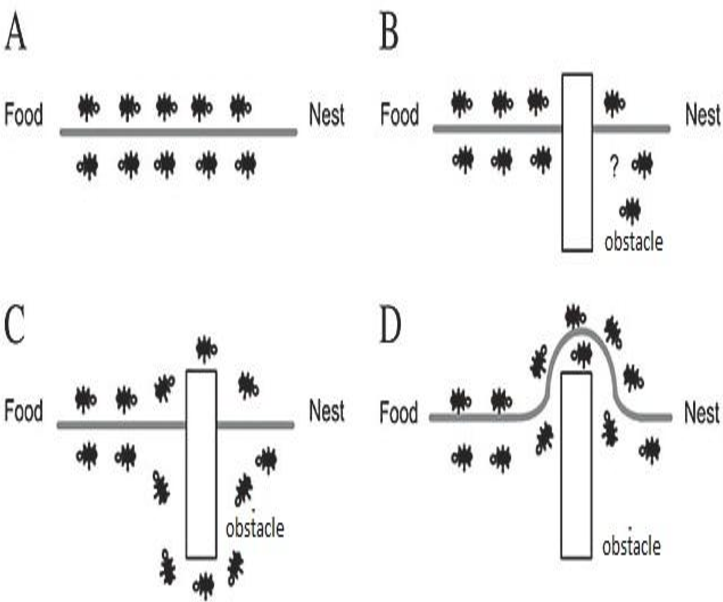
\includegraphics[scale=0.3]{aco_obstacle.png}
\end{center}
\caption{Ponašanje mrava u slučaju prepreke na putu do hrane}
\label{fig:mravi}
\end{figure}

Sama ideja algoritma oponaša spomeutno ponašanje mrava. Naime, uvodimo pojam ``mrava'' koji će se kretati po grafu i tražiti najkraći put. Algoritam će biti objašnjen na problemu trgovačkog putnika. Ono što je prednost datog algoritma jeste upravo ta što se može prilagoditi dinamičkoj situaciji.

\section{Primena ACO algoritma na TSP}
\label{acotsp}

\subsection{Problem trgovačkog putnika}
\label{subsec:podnaslov1}

Problem trgovačkog putnika je jedan od najpoznatijih problema iz grupe NP - teških problema diskretne i kombinatorne optimizacije. Pojam ``trgovački putnik'' prvi put je upotrebljen 1932. godine. U osnovi se svodi na to da trgovački putnik tačno zna koje gradove treba da poseti, takođe zna i kolika je međusobna udaljenost među gradovima. Jedini problem je taj što je u obavezi da poseti svaki grad samo jednom i da se vrati u grad iz kog je pošao. Rešenje problema se ogleda u tome da trgovački putnik odredi redosled gradova i da pritom putuje najoptimalnijom mogućom rutom, odnosno najkraćim i najbržim putem. Kretanje od grada do grada se odvija istom brzinom, odnosno kraći put je brži put. Na prvi pogled ovaj problem ne izgleda teško, ali ako se uzme u obzir da ima faktorijalnu složenost, računanjem se dobija da već za 10 gradova posotji 3,628,800 mogućih kombinacija obilaska gradova.

\subsection{ACO algoritam za TSP i parametri}
\label{subsec:podnaslov1}

U svakom koraku ACO algoritma, mrav se nalazi u nekom čvoru \textit{i} i treba da odabere naredni čvor \textit{j} u koji treba da pređe i to između onih čvorova koje na svom putu još uvek nije posetio. Verovatnoća preslaska u naredni čvor je određena rastojanjem između čvorova \textit{i} i \textit{j} kao i količinom feromona na grani koja ih spaja. Verovatnoća prelaska je data narednom formulom:

\begin{equation}\label{1}
p_{i,j}^k = {t_{i,j}^\alpha * distance_{i,j}^{-\beta} \over \sum_{l \in J_k}^{} t_{i,j}^\alpha * distance_{i,j}^{-\beta}}
\end{equation}

Ova formula predstavlja verovatnoću da će mrav \textit{k} u narednoj iteraciji algoritma preći u čvor \textit{j} iz čvora \textit{i}.


Promenljiva $t_{i,j}^\alpha$ predstavlja količinu feromona između čvorova \textit{i} i \textit{j}, dok $distance_{i,j}^{-\beta}$ predstavlja takozvanu vidljivost čvora \textit{j}  iz čvora \textit{i} i ona je definisana kao:

\begin{equation}\label{2}
distance_{i,j} = \frac{1}{d_{i,j}}
\end{equation}

gde $d_{i,j}$ predstavlja rastojanje između gradova \textit{i} i \textit{j}. Što je proizvod $t_{i,j} * distance_{i,j}$ veći to je veća i verovatnoća prelaska u grad \textit{j}. Trag feromona i vidljivost podignuti su na stepene $\alpha$ i $\beta$ respektivno. Ovi parametri kontrolišu uzajamnu bitnost informacija o tragu feromona $t_{i,j}$ nasuprot informacije o udaljenosti $distance_{i,j}$.

Nivo traga feromona mora da se ažurira nakon što svi mravi završe svoje kretanje kroz graf. Naredna formula predstavlja način na koji se trag feromona ažurira:

\begin{equation}\label{3}
t_{i,j} = (1-\rho) * t_{i,j} + \Delta t_{i,j}
\end{equation}

Faktor $\rho$ obezbeđuje da se feromon ne akumulira beskonačno i određuje količinu starog feromona koji će biti prenet u sledeću iteraciju algoritma.

\begin{equation}\label{4}
\Delta t_{i,j}  = \sum_{k=1}^{m} \Delta t^k_{i,j}
\end{equation}

U ovoj formuli \textit{m} predstavlja broj mrava, dok je $\Delta t^k_{i,j}$ kolicičina feromona koju je deponovao mrav k na poziciji između čvora \textit{i} i \textit{j}.

\section{Implementacija}
\label{sec:naslov1}

U samoj implementaciji korišćene su tri klase \textit{Graph}, \textit{ACS} i \textit{Ant}. 

Klasa \textit{Graph} sadrži neke opšte informacije o gradovima kao što su:
\begin{itemize}
  \item \textbf{distances}: predstavlja matricu rastojanja između gradova
  \item \textbf{rank}: predstavlja broj gradova, važi da između svaka dva grada postoji put
  \item \textbf{pheromone}: predstavlja matricu nivoa feromona između gradova 
\end{itemize}

\begin{figure}[h!]
\begin{center}
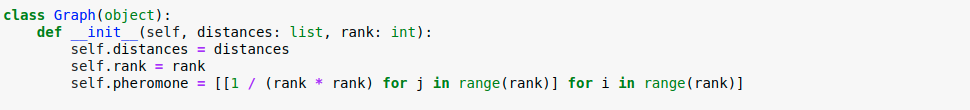
\includegraphics[width=1\columnwidth]{slika1.png}
\end{center}
\caption{Klasa Graph}
\label{fig:slika1}
\end{figure}

Klasa \textit{ACS} (eng.~{\em ant colony system}) je klasa koja se koristi za rešavanje problema putujućeg trgovca primenom ACO algoritma. Parametre koje sadrži su:

\begin{itemize}
	\item \textbf{generations}: predstavlja broj iteracija samog algoritma
	\item \textbf{ant\_count}: predstavlja broj mrava koji se kreira u svakoj iteraciji
	\item \textbf{alpha}: pozitivan parametar iz formule \ref{1} koji određuje uticaj feromona pri određivanju narednog čvora u koji mrav treba da pređe
	\item \textbf{beta}: pozitivan parametar iz formule \ref{1} koji određuje uticaj udaljenosti između gradova(čvorova) pri određivanju narednog čvora u koji mrav treba da pređe
	\item \textbf{rho}: pozitivan parametar iz formule \ref{3} koji oređuje koja količina starog feromona se prenosi u narednu iteraciju algoritma
	\item \textbf{Q}: pozitivan parametar
		
\end{itemize}


\begin{figure}[h!]
\begin{center}
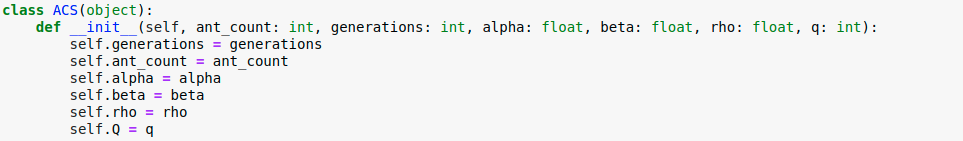
\includegraphics[width=1\columnwidth]{slika2.png}
\end{center}
\caption{Klasa ACS}
\label{fig:slika2}
\end{figure}


Ova klasa sadrži metode \textit{update\_pheromone} i \textit{solve}.
Metod \textit{update\_pheromone} vrši ažuriranje matrice feromona između gradova koristeći formule koje su objašnjene u \ref{subsec:podnaslov1}.


\begin{equation}
t_{i,j} = (1-\rho) * t_{i,j} + \Delta t_{i,j}
\end{equation}

\begin{equation}
\Delta t_{i,j}  = \sum_{k=1}^{m} \Delta t^k_{i,j}
\end{equation}

Polje \textit{i,j} matrice feromona se ažurira tako što se na već postojeću vrednost jačine feromona koja se umanjuje množeći se sa parametrom $\rho$, dodaje vrednost $\Delta t_{i,j}$ koja predstavlja sumu jačine feromona koju ostavlja svaki od mrava prolazeći tim putem.

\begin{figure}[h!]
\begin{center}
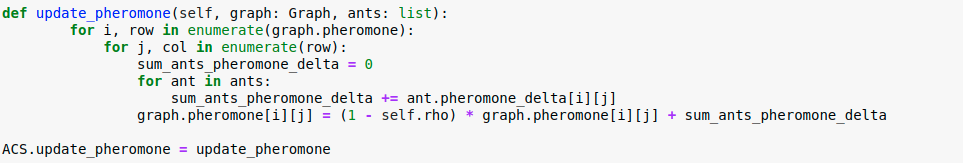
\includegraphics[width=1\columnwidth]{slika3.png}
\end{center}
\caption{Metod koji vrši ažuriranje feromona}
\label{fig:slika3}
\end{figure}


Metod \textit{solve} je od ključnog značaja za rešavanje problema trgovačkog putnika. Ovaj metod pronalazi najbolje rešenje u smislu najkraćeg puta koje trgovac treba da obiđe. Kao povratna vrednost same funkcije vraća se najbolje rešenje koje predstavlja putanju, odnosno čvorove grafa kao i cenu, odnosno dužinu puta. 

U prvoj petlji se prolazi kroz niz iteracija koja se zadaje kao parametar grafa. U svakoj iteraciji formiraju se instance mrava. Potom se za svakog mrava iz skupa mrava u petlji prolazi niz čvorova iz grafa pri čemu mrav svaki put posećuje čvor iz skupa neposećenih čvorova sve dok ne obiđe sve čvorove. Nakon završetka te petlje računa se ukupna cena pređenog puta za trenutno izabranog mrava. Ukoliko je trenutna ukupna cena manja od najbolje, ažurira se najbolja cena, takođe ažurira se i redosled posećenih čvorova kako bi se znao put kojim je mrav prošao. Na samom kraju svaki mrav ažurira količinu feromona koju je proizveo krećući se datim grafom, taj podatak se koristi pri ažuriranju matrice feromona na nivou iteracije. 

\begin{figure}[h!]
\begin{center}
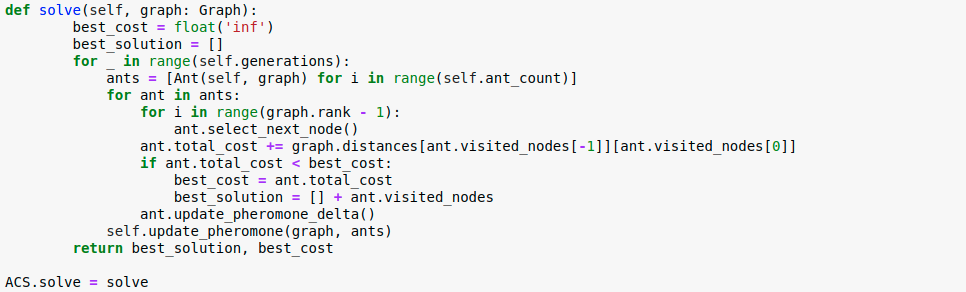
\includegraphics[width=1\columnwidth]{slika4.png}
\end{center}
\caption{Metod solve}
\label{fig:slika4}
\end{figure}

Klasa \textit{Ant} koja predstavlja jednog mrava u sistemu sadrži sledeće podatke o mravu:

\begin{itemize}
\item \textbf{colony}: instanca klase (eng.~{\em Ant Colony System}) u kome je mrav kreiran
\item \textbf{graph}: instanca grafa koji mrav obilazi
\item \textbf{total\_cost}: predstavlja cenu puta koji je mrav prešao
\item \textbf{visited\_nodes}: niz čvorova grafa koje je mrav obišao
\item \textbf{pheromone\_delta}: veličina feromona koju je mrav proizveo
\item \textbf{unvisited\_nodes}: predstavlja neposećene čvorove u grafu
\item \textbf{start\_node}: početni čvor iz kog mrav polazi u obilazak grafa
\item \textbf{visitied\_nodes}: predstavlja niz čvorova grafa koje je mrav obišao
\item \textbf{current\_node}: indeks čvora koji mrav obilazi

\end{itemize}



\begin{figure}[h!]
\begin{center}
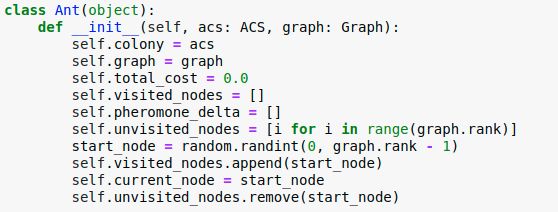
\includegraphics[width=1\columnwidth]{slika5.png}
\end{center}
\caption{Metod ant}
\label{fig:slika5}
\end{figure}

Ova klasa sadrži i dve metode \textit{select\_next\_node} i \textit{update\_pheromone\_delta}.
Metoda \textit{select\_next\_node} određuje naredni čvor u koji mrav treba da pređe prema formuli koja je objašnjena u \ref{subsec:podnaslov1}. 

\begin{equation}\label{1}
p_{i,j}^k = {t_{i,j}^\alpha * distance_{i,j}^{-\beta} \over \sum_{l \in J_k}^{} t_{i,j}^\alpha * distance_{i,j}^{-\beta}}
\end{equation}

\begin{figure}[h!]
\begin{center}
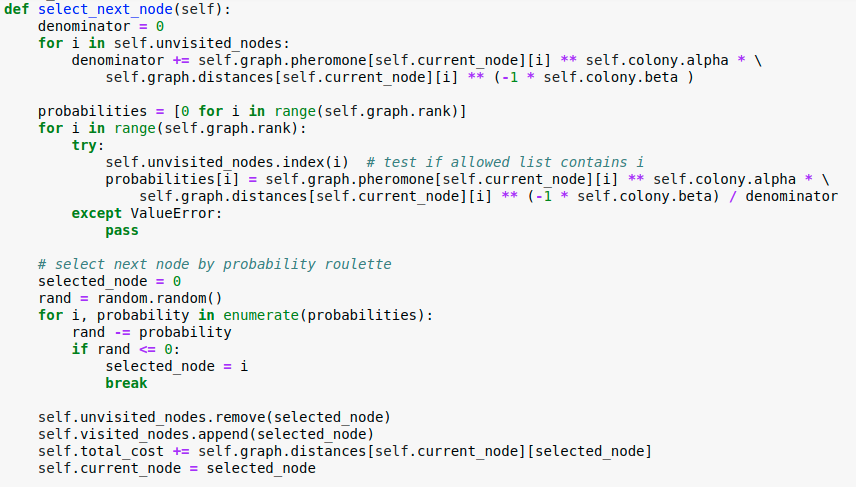
\includegraphics[width=1\columnwidth]{slika6.png}
\end{center}
\caption{Metod select\_next\_node}
\label{fig:slika5}
\end{figure}

Metoda \textit{update\_pheromone\_delta} vrši ažuriranje vrednosti feromona
za datog mrava u matrici pheromone\_delta.

\begin{figure}[h!]
\begin{center}
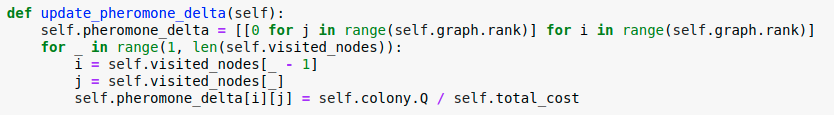
\includegraphics[width=1\columnwidth]{slika7.png}
\end{center}
\caption{Metod update\_pheromone\_delta}
\label{fig:slika5}
\end{figure}


%laEksperimentalno je dokazano da kada je broj mrava jednak maksimalnom broju gradova algoritam brže konvergira ka optimalnom rešenju nego kada se koristi veći broj mrava.

\addcontentsline{toc}{section}{Literatura}

\bibliography{seminarski} 
\bibliographystyle{plain}



\end{document}
